% This is a thesis template that attempts to conform to the guidelines
% published by UTRGV's Graduate School office.

% Please report any issues to
% https://github.com/UTRGV-SMSS/Thesis-Template/issues

% The author of this template is Guillermo Garza.
% Modified by Moises Castillo to conform to June 2018 updates.


% Switch this line to the final option when submitting your thesis.
% This will correct counts and remove labels that are shown during draft mode
%\documentclass[masters,draft]{UTRGVthesis}
\documentclass[masters,final]{UTRGVthesis}
%\documentclass[masters,final, nodedication, noacknowledgments]{UTRGVthesis}
%\usepackage{mathpazo}

% Set Custom font, requires XeLaTeX
%\setmainfont{Times New Roman}
%\setmainfont{Comic Sans MS}

% Load your packages below.
% Make hyperref and showkeys come at the end of your loaded packages
% to make sure they are not over-written.  They redefine many
% standard LaTeX commands
\usepackage{docmute} % for inputting complete documents. Useful for LyX users
\usepackage{booktabs} % for better tables
\usepackage{microtype} % for better typography
\usepackage[colorlinks=false]{hyperref}  % for urls
\usepackage{showkeys} % shows labels during draft mode
\usepackage[document]{ragged2e} % uncomment for non-justified text


% Uncomment the line below to check if text is aligned to margins
%\margins

% To change body font from Times Roman to Times New Roman, compile with XeLaTeX
% This assumes you have Times New Roman font installed in your machine
% WARNING! This will NOT change the font in Math Environments
\usepackage{ifxetex}
\ifxetex{}
   \usepackage{fontspec}
   \setmainfont{Times New Roman}
\fi

% This is to ease the use of bibliography from ADS
%  some journals choose to have their name abbreviated with a command
%  assuming the use of the AASTeX package. The following was a file from ADS
%       http://cdsads.u-strasbg.fr/abs_doc/aas_macros.sty
\usepackage{aas_macros}

\usepackage{siunitx} % for proper units

% this sets hanging indention for bibliography
\usepackage[sort&compress]{natbib}      % for bibliography

\setlength\bibindent{2em}

\makeatletter
\renewcommand\NAT@bibsetnum[1]{\settowidth\labelwidth{\@biblabel{#1}}%
   \setlength{\leftmargin}{\bibindent}\addtolength{\leftmargin}{\dimexpr\labelwidth+\labelsep\relax}%
   \setlength{\itemindent}{-\bibindent}%
   \setlength{\listparindent}{\itemindent}
\setlength{\itemsep}{\bibsep}\setlength{\parsep}{\z@}%
   \ifNAT@openbib
     \addtolength{\leftmargin}{\bibindent}%
     \setlength{\itemindent}{-\bibindent}%
     \setlength{\listparindent}{\itemindent}%
     \setlength{\parsep}{0pt}%
   \fi
}
\makeatother

% this sets the name of the bibliography
% add \vspace{1cm} here to adjust vertical spacing after bibliography title
\renewcommand{\bibname}{BIBLIOGRAPHY}

% Insert your name and major here in the format shown
\Author{Moises Castillo}
\AuthorLastFirst{Castillo, Moises}
\Major{Physics}


% Insert your graduation date here
\Month{August}
\Year{2019}


% Insert the title of your thesis here.
% If you have a long title, split it between multiple lines using the \\ command
% Also, use comment characters to avoid unwanted spaces in the Abstract page
\Title{Pipeline for variable star detection and\\
eclipsing binary characterization}


% Insert your research advisor and his title here
\Advisor{Dr.\ Mario C.\ Diaz}
\AdvisorTitle{Chair of Committee}

% Insert the members of your committee here
% You can also give MemberA a special title
\MemberA{Dr.\ Nicolas Pereyra}  %\MemberATitle{Co-Chair of Committee}
\MemberB{Dr.\ Andreas Hanke}
\MemberC{}
\MemberD{}
\MemberE{}


% Insert the text of your abstract below.
% The bibliography style "citation" required by the manual is automatically
% generated.  Specify the "final" option in the \documentclass to update the
% counts to the correct values.
\Abstract{%
The purpose of this project is to create a pipeline written in python that creates a framework for detecting variable stars by
creating a catalogue of stars and light curves of data from eclipsing binary star observations.
The eclipsing binary stars were the main targets in the observations and will be characterized.
}


% You can dedicate your paper here.  This is optional.
\Dedication{%
    Dedication should be simple, in good taste, and fit on one page.
}


% Acknowledge those who helped and supported you here. This is optional.
\Acknowledgments{%
    Acknowledgements should be simple, in good taste, and fit on one page. CTMO, CGWA
}


% Insert your biographical sketch here.
\BiographicalSketch{%
    A brief biographical sketch of the student is required as part of each thesis.
}



\begin{document}

% This starts page counting in Roman numerals
\frontmatter


% This command makes the formal preliminary pages.
% You can comment it out during the drafting process if you want to save paper.
\makepreliminarypages{}

% These insert a table of contents, list of tables, and list of figures
\tableofcontents
\listoftables
\listoffigures


% This starts regular page counting in Arabic numerals
\mainmatter{}

% This starts double-spaced text.  Opposite command is \singlespacing
\doublespacing{}


% OK. Everything is set up. Insert your thesis below.
% It's a good idea to split your thesis up into different files and use
% the \input command
\chapter{Introduction}
\label{ch:intro}

\section{Variable stars}
Stars are called variable when there is a detectable change in brightness or color on time scales of the order
of the mean life time of humans~\cite{percy_2007, sterken_1996}.
The first claimed documented variable star is Algol visible with the unaided eye.
There exists ancient Egyptian calendars of lucky and unlucky days that possibly contain the periodicity of Algol\cite{porceddu_2008, porceddu_2018}.
The Cairo Calendar dated to 1244--1163 BC has been shown by Porceddu et al.~\cite{porceddu_2015} to represent Algol as Horus, a sky god and
symbol of kingship,
as seen in the figure~\ref{fig:horus} by matching the actions of Horus and the events witnessed by an observer of Algol.

\begin{figure}[h]
    \centering
    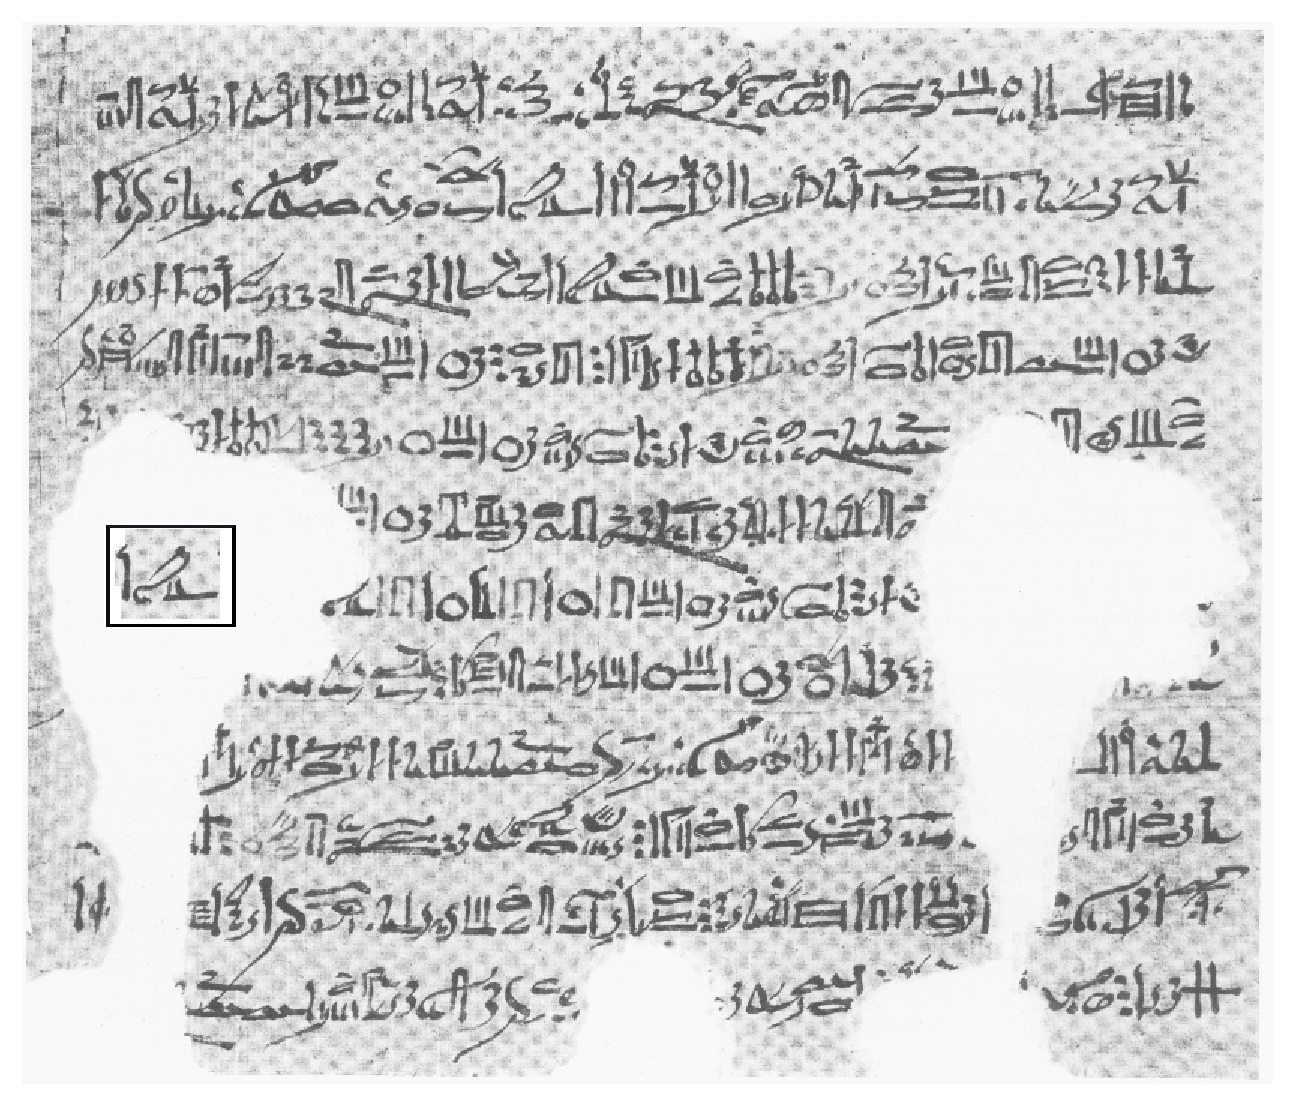
\includegraphics[width=\columnwidth]{figures/horus.eps}
    \caption{Inside the rectangle is the hieratic writing for the word Horus~\protect\cite{porceddu_2015}.}
\label{fig:horus}
\end{figure}

There is some curious relation between ancient Greek stories of the Gorgon Medusa, Perseus, the corresponding constellations, 
and the variable stars Algol and Omicron Ceti or more commonly named Mira (the wonderful).
Wilk~\cite{wilk_1996} suggests that the variability and location in the sky is embedded within the stories themselves.

The first recognized documented variable star, Omicron Ceti,  was recorded in 1596 and again in 1609 by David Fabricius while observing Jupiter.
Fabricius had first recorded Omicron Ceti as a nova, a singular event observed as a bright flash and quick dimming over the next few days,
comparing its significance with a supernova recorded by Tycho Brahe in 1572.
In 1638, Omicron Ceti was rediscovered by Johannes Phocylides Holwarda who found the periodic nature of this star to be approximately 11 months~\cite{hockey_2007}.

%In order to characterize eclipsing binary systems a light curve must be made.
%A light curve is a time series plot of the measured magnitude.

\section{Classifying variability}
Over time there have been several attempts to classify variable stars.
Classification systems reflect the current understanding of the mechanisms behind variability.
The earliest variable star observers like Goodricke and Pigott, who was employed to verify the variability of stars~\cite{pigott_1785}, would try to make sense of the observations and periods recorded by comparing and grouping different stars to those like Algol and $\omicron$ Ceti.  

One of the first attempts that went into detail was made by E.\ C.\ Pickering~\cite{sterken_1996, hoffleit_1972} in 1881 where he classified variable stars into the following categories\cite{pickering_1881}:
\begin{description}
    \item [Type I] Temporary stars. Examples, Tycho Brahe's star of 1572, new star in Corona, 1866.
    \item [Type II] Stars undergoing great variations in light in periods of several months or years. Examples, $\omicron$ Ceti and $\chi$ Cygni.
    \item [Type III] Stars undergoing slight changes according to laws yet unknown
    \item [Type IV] Stars whose light is continually varying, but the changes are repeated with great regularity in a period not exceeding a few days. 
    \item [Type V] Stars which every few days undergo for a few hours a remarkable diminution in light, this phenomenon recurring with great regularity. 
\end{description}

As time passes with more observations of variable stars, the collective understanding of the mechanisms of variability are improved.
With an improved understanding of physical processes including stellar evolution, pulsation, rotation, and eclipsing, then the taxonomy of classes is refined.

Since 1946, on behalf of the International Astronomical Union (IAU), Moscow variable star researchers have compiled detailed catalogs and certified 
variable stars in the General Catalogue of Variable Stars (GCVS). 
GCVS 5.1 is the most current version of the catalog containing $52,011$ variable objects discovered and named as variable stars by 2015~\cite{samus_2017}.

\subsection{General Catalogue of Variable Stars 5.1 Variability Types}
Variability types are in groups according to the major astrophysical reasons for variability.
The variable types have letter designations that typically corresponds to the original star that is observed with the same type of variability.
For example, in the eruptive group there is a type called GCAS that signifies eruptive irregular variables of the Gamma Cas type.
The definitions of the variable types are given by GVCS and maintained on their
website: \url{http://www.sai.msu.su/gcvs/gcvs/}

The following are groups with the variable types in those groups.
The reader can visit the GCVS Variability Types webpage\footnote{GCVS Variability Types: \url{http://www.sai.msu.su/gcvs/gcvs/vartype.htm}} to 
see specific variable types. 
\begin{description}
    \item [eruptive] FU, GCAS, I, IA, IB, IN, INA, INB, INT, IT, IN (YY), IS, ISA, ISB, RCB, RS, SDOR, UV, UVN, WR,
    \item [pulsating] ACYG, BCEP, BCEPS, CEP, CEP (B), CW, CWA, CWB, DCEP, DCEPS, DSCT, DSCTC, GDOR, L, LB, LC, M, PVTEL, RPHS, RR, RR (B), RRAB,
           RRC, RV, RVA, RVB, SR, SRA, SRB, SRC, SRD, SXPHE, ZZ, ZZA, ZZB,
    \item [rotating] ACV, ACVO, BY, ELL, FKCOM, PSR, SXARI,
    \item [cataclysmic (explosive and novalike) variables] N, NA, NB, NC, NL, NR, SN, SNI, SNII, UG, UGSS, UGSU, UGZ, ZAND,
    \item [eclipsing binary systems] E, EA, EB, EW, GS, PN, RS, WD, WR, AR, D, DM, DS, DW, K, KE, KW, SD,
    \item [intense variable X-ray sources] X, XB, XF, XI, XJ, XND, XNG, XP, XPR, XPRM, XM,
    \item [other symbols] BLLAC, CST, GAL, L:, QSO, S, *, +, $\colon$
    \item [the new variability types] ZZO, AM, R, BE, LBV, BLBOO, EP, SRS, LPB
\end{description}

This document will not cover all the different variable stars types. 
The study specifically will focus on EW type eclipsing binary systems.  

%%%% CONSIDER OMISSION 
%% \section{Characterizing variability}
%% Using different algorithms one can distinguish the difference between the types of variable star system.
%% 
%% This demonstrates RR Lyrae
%% This demonstrates Eclipsing binaries
%% 
%% The relation between orbital mechanics and light curves
%% 
%% This demonstrates solar spots
%% 
%% Complex systems can involve a combination of these different systems.

\chapter{Eclipsing binary systems}
\label{chp:ebsystems}

\section{Defining eclipsing binary system}
As the name implies, an eclipsing binary system is such that at least two objects orbit close to the
same plane as viewed from an observer on Earth so that one object eclipses the other.

\section{Eclipsing binary system types}
Eclipsing binary systems are classified into three sub group types.
The following are the eclipsing binary system types and definitions set by the GCVS$\colon$
\subsection{Classification based on the shape of the light curve}
\begin{description}
    \item[E]   Eclipsing binary systems. These are binary systems with orbital planes so close to the observer's line of sight (the inclination i of the orbital plane to the plane orthogonal to the line of sight is close to 90 deg) that the components periodically eclipse each other. Consequently, the observer finds changes of the apparent combined brightness of the system with the period coincident with that of the components' orbital motion.

    \item[EA]   Algol (Beta Persei)-type eclipsing systems. Binaries with spherical or slightly ellipsoidal components. It is possible to specify, for their light curves, the moments of the beginning and end of the eclipses. Between eclipses the light remains almost constant or varies insignificantly because of reflection effects, slight ellipsoidality of components, or physical variations. Secondary minima may be absent. An extremely wide range of periods is observed, from 0.2 to >= 10000 days. Light amplitudes are also quite different and may reach several magnitudes.

    \item[EB]   Beta Lyrae-type eclipsing systems. These are eclipsing systems having ellipsoidal components and light curves for which it is impossible to specify the exact times of onset and end of eclipses because of a continuous change of a system's apparent combined brightness between eclipses; secondary minimum is observed in all cases, its depth usually being considerably smaller than that of the primary minimum; periods are mainly longer than 1 day. The components generally belong to early spectral types (B-A). Light amplitudes are usually <2 mag in V.

    \item[EP]    Stars showing eclipses by their planets. Prototype: V0376 Peg.

    \item[EW]   W Ursae Majoris-type eclipsing variables. These are eclipsers with periods shorter than 1 days, consisting of ellipsoidal components almost in contact and having light curves for which it is impossible to specify the exact times of onset and end of eclipses. The depths of the primary and secondary minima are almost equal or differ insignificantly. Light amplitudes are usually <0.8 mag in V. The components generally belong to spectral types F-G and later.
\end{description}

\subsection{Classification according to the components' physical characteristics}
\begin{description}
    \item[GS]   Systems with one or both giant and supergiant components; one of the components may be a main sequence star.

    \item[PN]   Systems having, among their components, nuclei of planetary nebulae (UU Sge).

    \item[RS]   RS Canum Venaticorum-type systems. A significant property of these systems is the presence in their spectra of strong Ca II H and K emission lines of variable intensity, indicating increased chromospheric activity of the solar type. These systems are also characterized by the presence of radio and X-ray emission. Some have light curves that exhibit quasi sine waves outside eclipses, with amplitudes and positions changing slowly with time. The presence of this wave (often called a distortion wave) is explained by differential rotation of the star, its surface being covered with groups of spots; the period of the rotation of a spot group is usually close to the period of orbital motion (period of eclipses) but still differs from it, which is the reason for the slow change (migration) of the phases of the distortion wave minimum and maximum in the mean light curve. The variability of the wave's amplitude (which may be up to 0.2 mag in V) is explained by the existence of a long-period stellar activity cycle similar to the 11-year solar activity cycle, during which the number and total area of spots on the star's surface vary.

    \item[WD]   Systems with white-dwarf components.

    \item[WR]   Systems having Wolf-Rayet stars among their components (V 444 Cyg).
\end{description}

\subsection{Classification based on the degree of filling of inner Roche lobes}
\begin{description}
    \item[AR]   Detached systems of the AR Lacertae type. Both components are subgiants not filling their inner equipotential surfaces.

    \item[D]   Detached systems, with components not filling their inner Roche lobes.

    \item[DM]   Detached main-sequence systems. Both components are main-sequence stars and do not fill their inner Roche lobes.

    \item[DS]   Detached systems with a subgiant. The subgiant also does not fill its inner critical surface.

    \item[DW]   Systems similar to W UMa systems in physical properties (KW, see below), but not in contact.

    \item[K]   Contact systems, both components filling their inner critical surfaces.

    \item[KE]   Contact systems of early (O-A) spectral type, both components being close in size to their inner critical surfaces.

    \item[KW]   Contact systems of the W UMa type, with ellipsoidal components of F0-K spectral type. Primary components are main-sequence stars and secondaries lie below and to the left of the main sequence in the (MV,B-V) diagram.

    \item[SD]   Semidetached systems in which the surface of the less massive component is close to its inner Roche lobe.
\end{description}

The combination of the above three classification systems for eclipsers results in the assignment of multiple classifications for object types. These are separated by a solidus (``/'') in the data field. Examples are: E/DM, EA/DS/RS, EB/WR, EW/KW, etc.


\section{Eclipsing Binary Characterization}
Binary stars can reveal physical properties by examining the light curves.

\section{Light curve}
A light curve is a plot of brightness vs time. 
Variations in brightness must be allowed due to changes in the optical path rather than
from the source.
The specific methods on considering the tolerance will be discussed in Chapter~\ref{chp:data}.

The method for calculating the physical parameters from light curve data that is commonly used in
eclipsing binary research is called WD Code.

\section{WD code}
Current models use a process first developed by Wilson and Devinney in 1971~\cite{wilson_devinney_1971}
for studying close eclipsing binary systems now called WD code.

In this study a modified WD code is used called PHOEBE (Physics of Eclipsing Binaries) code.
The current release PHOEBE 2.1~\cite{horvat_2018} was built upon the previous releases 2.0~\cite{prsa_2016}
and the original legacy code~\cite{prsa_2005}. 


\subsection{Modified WD code}


\section{O-C calculations}
Observed minus Calculated

\section{Equations of motion}




\chapter{Instrumentation}
\section{Dome}
Dr.Cristina Valeria Torres Memorial Observatory inaugurated May 5, 2018.
Formerly Nompuewenu Observatory.
Custom build.
\subsection{Specifications}
\subsection{Robotizing of dome}
\subsection{Hardware}
\begin{enumerate}
    \item Arduino *Need to Specify* 
    \item Yaskawa J1000 Drive
\end{enumerate}

\section{Telescope System}
\subsection{16-inch Meade LX200-GPS}
\subsubsection{Specifications}
\subsubsection{Installation}
\subsubsection{Limitations}

\subsection{CDK17 on L-500 direct drive mount}
\subsubsection{Specifications}
\subsubsection{Installation}
\subsubsection{Limitations}

\section{Camera}
\subsection{SBIG STF-8300}
\subsubsection{16-inch Meade}

\subsection{Apogee Alta F16M}
\subsubsection{16-inch Meade}
\subsubsection{CDK17}

\section{Software}
\subsection{Dome}
\subsection{Telescope}
\subsection{Camera}
\subsection{Observatory Control}
This section explains the different observatory control systems implemented during use.
Observatory controls unify the different hardware and software. 
\subsubsection{POTH}
\subsubsection{INDI}

\chapter{Methods}
\label{chp:data}

\section{Data Acquisition}
Eclipsing binary optical data acquisition requires an observer to do time series ccd photometry
of one target with an observation cadence dependent on the period of the system.
For example, the data gathered for this project was collected on multiple nights and observed on the order of hours with evenly timed frames.

\subsection{Planning Observations}
There are some options for selecting sources to observe.
The following process is one learned in practice with amateur astronomer Carlos Colazo of Argentina.
This study uses the Variable Star and Exoplanet Section of Czech Astronomical Society's observation project called
BRNO Regional Network of Observers (BRNO)~\cite{brno}.

An ephemeris is made by using a table of predicted times of minima published on the BRNO webpage.
For site specific predictions, the webpage needs to be visited in the original Czech language.
A web form shown in figure~\ref{fig:brno} appears to include latitude and ELongitude (longitude in degrees east of the meridian) of the observation site.
\begin{figure}[h]
    \centering
    \includegraphics[width=\columnwidth]{example-image}%{figures/brno.png}
    \caption{Web form for eclipsing binary predicted times of minima from the Variable Star and Exoplanet Section of Czech Astronomical Society's observation project called BRNO Regional Network of Observers (BRNO)}
\label{fig:brno}
\end{figure}

It is important to mention the American Association of Variable Star Observers (AAVSO)
offers a target tool on the web~\footnote{\url{https://filtergraph.com/aavso}} to help make an observation plan.


\subsubsection{Selection criteria}
Typically, EW type binary stars have the shortest period and were chosen for this reason. 
Observation time is set to start no later than one hour before the predicted time of minima.
The error on the predicted time of minima can be great due to lack of observational data.

BRNO classifies stars using a scale from 1 to 10.
As a rule of thumb, the scale refers to the number of years since last reported observation.
BRNO explicitly recommends observers observe objects with a rating of 5 or more.

Since observation are made over several hours it is best practice to pick objects on the eastern parts of the sky.
This allows for maximum viewing time. The altitude of the target should be above 30 degrees for proper photometry study, but 
can be slightly lower.

Lastly, as with all observations, the limiting magnitude of the system will dictate what objects are observable.
The change in magnitude of known eclipsing binaries stated in catalogs.
The observer must make certain that the instrumentation allows for such observation.
Millimagnitude precision is standard in exoplanet research, but is not required for any of the observations in this study.

\subsection{Observation}
When performing an eclipsing binary observation the observer should attempt to observe 
the same binary system through the entire night to capture the most complete period. 
Some systems need to be observed across several nights to obtain a full period.
When conducting any measurement it is good practice to make plots on-the-fly to make sure the quality of data is consistent.

Since the observer typically will begin observation on the eastern sky with a low altitude, the air mass will be highest
at the beginning of the observation.
This can present a problem if the observer does not consider the increase of flux as the object approaches zenith or the highest
point in the sky.
When the object being observed reaches zenith, the air mass is the lowest and if not considered can cause over saturation of the CCD\@.
Saturation is when the potential well for the pixel is completely filled and will no longer capture the electrons
converted from the photon interaction with the CCD\@.

\subsection{Post observation}
After the observation is complete it is vital to collect calibration frames required for proper data reduction for photometry.
Data reduction is the process for removing noise due to dark current, bias, and any obscuring defects in the optical path of the system.
Required calibration frames are,
\begin{description}
    \item[Flat Frames] Flat frames are made by using an evenly illuminated light source. This can be created by using a white screen
        and a diffuse white light. This process will show any obscuring defects that are in the optical path like dust and vignetting.
        The required exposure time depends on the lighting system to reach a signal between 30 to 50 percent of saturation.
    \item[Dark Frames] Dark frames are made by taking closed `exposures' of the CCD\@. Exposure time for the dark frames need to match
        the flat frame exposure times and object exposure times.
    \item[Bias Frames] Bias frames are only needed if the observer does not match the dark frame exposure times to the flat frames.
\end{description}

\section{Motivation for pipeline: lightcurator}
Observing eclipsing binary systems especially of EW type require an observer to track the source on the order of hours.
This means the data produced can include various stars as well as some potentially undiscovered variable stars.
For this reason, the author created a python package called 
\textit{lightcurator}~\cite{castillo_2019} which is publicly available on Github \url{https://github.com/moemyself3/lightcurator}
and on PyPI \url{https://pypi.org/project/lightcurator/} for easy installation using the package insaller for Python, \textit{pip}.
Lightcurator includes 2 packages: \textit{lightcurve} and \textit{calibration}.
The functions included are described in the sections that follow.

\section{Pipeline for variable star detection}
\begin{enumerate}
    \item Reduce data
    \item Align frames
    \item Create deepsky frame
    \item Plate solve deepsky
    \item Extract sources from deepsky frame
    \item Extract sources from aligned frames
    \item Cross match sources from aligned frames to deepsky frames
    \item Cross match master catalog with catalogs like VSX and GCVS
    \item Create Database of known sources
    \item Correct or normalize extracted flux data
    \item Plot individual light curves
    \item Analyze individual light curves for variability estimation
    \item Sort database given variability ranking
\end{enumerate}

\subsection{Data reduction}
Reading, writing fits files, and creating data tables is done with a python
package called \textit{astropy}~\cite{astropy_2013,astropy_2018}.
Majority of the data reduction is done with astropy core package,
coordinated packages, and affiliated packages.
Coordinated packages are maintained by the Astropy Project
and affiliated packages are not maintained by the Astropy Project,
but is a part of the Astropy Project community.

Coordinated packages in use are \textit{astroquery}~\cite{astroquery}, \textit{ccdproc}~\cite{ccdproc}, \textit{photutils}~\cite{photutils}.
An affiliated package in use is \textit{astroscrappy}~\cite{astroscrappy}.
A package in the process of becoming an official affiliated package that is in use is \textit{astroalign}. 
More details of astroalign are discussed in Section~\ref{section:align} 

\subsubsection{Calibration}
Lightcurator has a module called calibration that provides the tools for convenient data reduction.
The routine begins with the creating of the list of the fits files to be used
with \textit{ccdproc.ImageFileCollection}.
The list is used for quick reference to all the fits files to be processed.
The \textit{validate\_units} function checks for the fits keyword `BUNIT'. 
If the units are missing then the function raises an exception and suggests
to the user to use the \textit{add\_units} function. 
All the data sets including flats and darks collected at CTMO are missing units.
This function inserts the `BUNIT' keyword and sets the value to `adu'.

After defining the paths to the location of the calibration files, i.e.\
flats and darks, running \textit{create\_masters} makes a master dark and master flat frame.
This is done by doing a median combine of the dark frames. 
The dark frames are a measure of dark current which is the noise generated by the thermal energy generated by the silicon of the CCD\@.
Since the CCD has a constant voltage applied across the device, there is a bias in the signal generated that contains some read noise.
By taking dark frames at the same exposure time as flat frames, then bias frames can be ignored since the noise will also be removed along
with the dark frame.



The function \textit{reduce} takes a user defined read noise, gain, and
path to the directory containing the data to be reduced. 
The \textit{reduce} function gain corrects the master dark and master flat, then
uses \textit{ccdproc.ccd\_proccess}. 
The \textit{ccdproc.ccd\_process } is an all-in-one function that gain corrects,
dark subtracts, and flat corrects. It can also take into considerations 
uncertainties for error propagation, over scan regions, and any trimming that
may be required in different set ups.
The new reduced fits frames are then saved to file for later processing.

Through this process it is important to note that the file goes from storing
16-bit data to 64-bit data.
This can easily cause a significant impact on a systems storage
since the new frames are about 4 times larger than before.

\subsubsection{Cosmic ray detection}
It is not uncommon to have cosmic rays hit the CCD causing peaks in signals that may be confused as sources during source extraction.
The final step in data reduction is cosmic ray detection.
For this, the function \textit{ccdproc.cosmicray\_lacosmic} identifies cosmic rays by identifying pixels based on a variation of
Laplacian edge detection described by van Dokkum~\cite{lacosmic} and implemented by McCully in \textit{astroscrappy}~\cite{astroscrappy}.
Lightcurator uses this algorithm with a function called \textit{hotpixfix} prior to alignment of frames to allow a flexible
approach by using raw frames instead of properly reduced frames.

\subsection{Align frames}
\label{section:align}
Frame alignment is done with a python package called \textit{astroalign} written by Dr.\ Martin Beroiz~\cite{beroiz_2019} which is publicly
available on Github\footnote{For the latest version of astroalign check: \url{https://github.com/toros-astro/astroalign}}

Astroalign is the preferred method for image alignment since the raw data frames do not have World Coordinate System (WCS) information attached to
the headers.
WCS information encodes the transformations required to change $x,y$-pixel location to right ascension (RA) and declination (DEC).

Lightcurator uses a function called \textit{try\_register} to catch exceptions and reject by truncating the data frame if alignment
cannot be completed.
Exceptions from astroalign that are most commonly experienced are \textit{MaxIterError} which is raised when the maximum number of iterations
allowed by astroalign are met and a custom \textit{Exception} raised when there are less than 3 sources detected.

\subsection{Create deepsky frame}
To create a deepsky frame a simple addition of all aligned frames are made.
The CCD data is loaded into python as CCDData of numpy.ndarray types.
Simple addition is used since the deepsky frame is only used for source detection and not for photometry.
A more appropriate method for combining frames would be a median combine. 

\subsection{Extract sources}
Source extraction is done with a python package called \textit{photutils}.

\subsection{Source cross matching}
Source cross matching is done with a python package-called 

\subsection{Analyzing variability}
Variability analysis is done with a python package called feets written by J Cabral~\cite{cabral_2018}


\section{Observed objects}
\begin{table}
    \centering
    \begin{tabular}[h]{l c c c}
    \toprule
    Target      & Type  & Filter    & Observation date \\ \bottomrule
    RV Vir      & M     & C         & 2017/02/23 \\ \midrule
    MQ Boo      & EB    & C         & 2017/04/26 \\ \midrule
    PR Boo      & EW    & C         & 2017/03/30 \\ \midrule
                &       & C         & 2017/04/20 \\ \midrule
                &       & C         & 2017/05/11 \\ \midrule
    Alp Boo     & ``???''   & RGB       & 2017/04/05 \\ \midrule
    EQ Uma      & EW/KW & CRGB      & 2017/04/06 \\ \midrule
    HP Aur      & EA    & C         & 2017/04/13 \\ \midrule
    NY Lyr      & EW/KW & C         & 2017/07/06 \\ \midrule
    AW Ari      & EW    & GB        & 2017/10/12 \\ \midrule
    SS Ari      & EW    & C         & 2016/11/27 \\ \midrule
                &       & RGB       & 2017/11/01 \\ \midrule
    XX LMi      & EW    & RGB       & 2018/03/20 \\ \midrule
    V467 Lyr    & EW:/KE:& CRG   & 2018/06/07 \\ \midrule
    V2793 Ori   & EA    & RGB   & 2017/11/17 \\
    \bottomrule
    \end{tabular}
    \caption{Observations of eclipsing binaries. Filters: RGB corresponds to Baader CCD RGB filters and C is unfiltered}\label{tab:observations}
\end{table}
\section{Known information of targets examined}



% This makes the bibliography.
% Enter your references in the BibTex file "references.bib"
% You can find bibtex info from Google Scholar.
%\bibliographystyle{siam}
\bibliographystyle{plain}
\bibliography{msthesisref}


% Uncomment the \appendix macro below for appendices
% Insert appendix chapters after the macro
%\appendix


% This inserts your Biographical Sketch
\biographypage{}

\end{document}
